\documentclass{article}
\usepackage[left=2cm,right=2cm,top=2cm,bottom=2cm]{geometry}
\usepackage[utf8]{inputenc}
\usepackage[german]{babel}
\usepackage{amsmath}
\usepackage{dsfont}
\usepackage[export]{adjustbox}
\usepackage{amsthm}
\usepackage{color}
\usepackage{amsfonts}
\usepackage{amssymb}
\usepackage{wasysym}
\usepackage{makeidx}
\usepackage{graphicx}
\usepackage[colorlinks=true,urlcolor=blue,linkcolor=blue]{hyperref}
\usepackage{ziffer}
\usepackage{minted}
\usepackage{xcolor}
\usepackage{framed}
\usepackage{mdframed}
\usepackage{subfiles}
\usemintedstyle{emacs}

\definecolor{purp}{HTML}{9A72AC}
\definecolor{re}{HTML}{FC6255}
\definecolor{gre}{HTML}{83C167}
\definecolor{blu}{HTML}{58C4DD}
\definecolor{shadecolor}{rgb}{0.85,0.85,0.85}
\definecolor{bg}{rgb}{0.95,0.95,0.95}
\setlength{\parindent}{0em} 

\BeforeBeginEnvironment{minted}{\begin{mdframed}[linewidth =2 ,backgroundcolor=bg , linecolor=black, linewidth=0.5]}
\AfterEndEnvironment{minted}{\end{mdframed}}

\newtheorem{defi}{Definition}
\BeforeBeginEnvironment{defi}{\begin{mdframed}[linewidth =2 ,backgroundcolor=bg , linecolor=black, linewidth=0.5]}
\AfterEndEnvironment{defi}{\end{mdframed}}

\newcommand{\bsp}{\textbf{Beispiel}:}
%\newcommand{\task}{\textbf{Aufgabe}:}

\newcommand{\bol}[1]{\textbf{#1}}
\newcommand{\q}[1]{\glqq #1\grqq}
\newcommand{\DODO}[1]{\textbf{\textcolor{red}{DODO:}} #1 \\ \begin{center}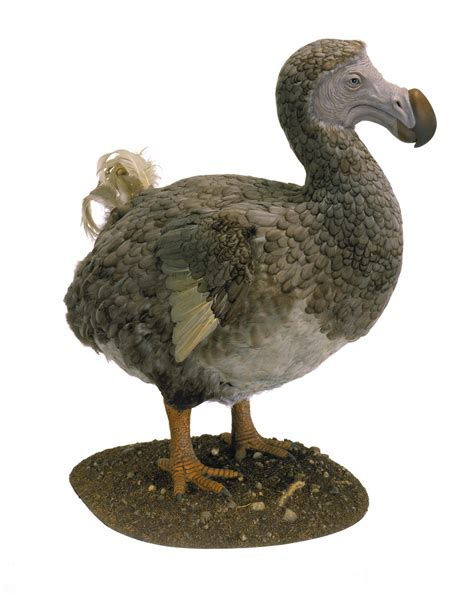
\includegraphics[scale=0.2]{../../media/dodo.jpg} \end{center}}

\newenvironment{task}[1]{
    \begin{shaded*}
    \textbf{Aufgabe #1}:
}{
    \end{shaded*}
}

\begin{document}
\subsection{Grundlagen}
Das Feld ist nicht die einzige Möglichkeit eine Liste zu implementieren. Die sogenannte 
verkettete Liste ist ebenfalls ein übliches Konzept. \\
Die \textbf{\color{red}grundlegende Idee} ist dabei folgende:
\begin{center}
    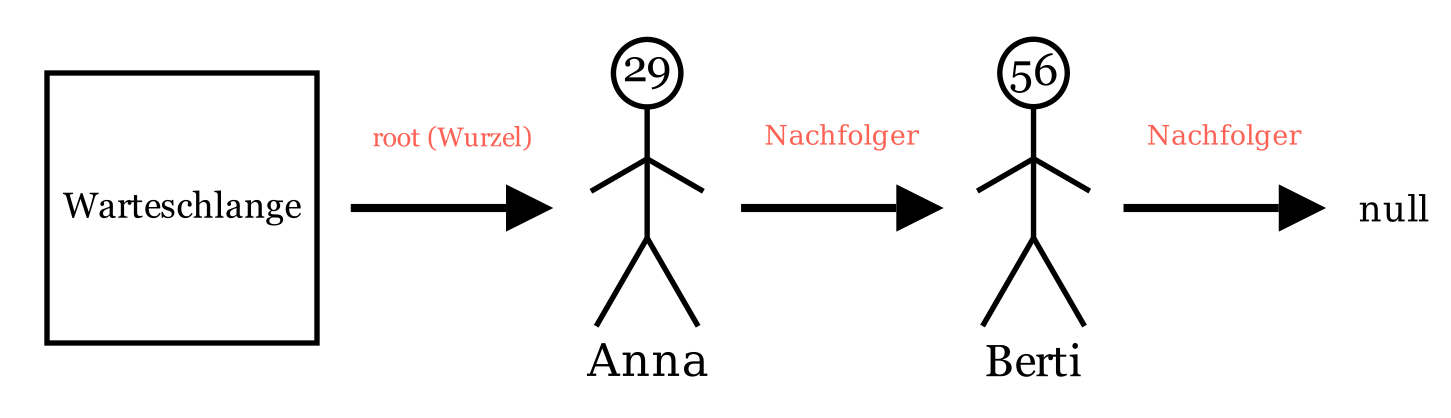
\includegraphics[scale=0.25]{../../media/linked_idea.png}
\end{center}
Die Klasse \textcolor{orange}{Warteschlange} organisiert unseren Zugriff und dient als Steuerzentrale für alle Methoden, die 
wir auf der Liste ausführen wollen. Die eigentlichen Listenelemente sind jetzt aber nicht mehr in einem 
Feld gespeichert, sondern sind eigene Objekte, die jeweils nur ihren Nachfolger kennen. Nicht einmal die 
Warteschlange selbst kennt alle Menschen (oder auch nur deren Zahl). Sie kann nur auf den ersten in der Schlange
zugreifen, die Wurzel (oder auch Anfang der Liste, im Englischen: root). Diese Idee scheint auf den ersten 
Blick umständlich, denn man kann nun nicht mehr auf ein beliebiges Listenelement zugreifen. \\
Tatsächlich hat diese verkettete Struktur aber andere Vorteile, die später noch deutlich werden. Ein 
offensichtlicher Vorteil ist aber die \textbf{Erweiterbarkeit}. Unsere Warteschlange kann jetzt nicht mehr 
voll laufen (außer unser Speicher ist voll), sondern wir können einfach weitere Menschen hinten anfügen, indem
wir dem letzten Listenelement (hier der Mensch Berti) eine Referenz auf seinen neuen Nachfolger geben. \\
\textit{Hinweis:} Sieht man sich die Struktur genau an, so wird klar, dass Berti nicht einmal von der 
Existenz Annas weiß, d.h. von seiner Vorgängerin. Dies nennt man ein \textbf{einfach verkettete} Liste.
Werden Referenzen in beide Richtung gesetzt, so ist es eine \textbf{doppelt verkettete} Liste. Oft 
genügt aber die Referenz in eine Richtung. 
Zusammengefasst in einem Klassendiagramm lautet unser aktuelles Ziel also: 
\begin{center}
    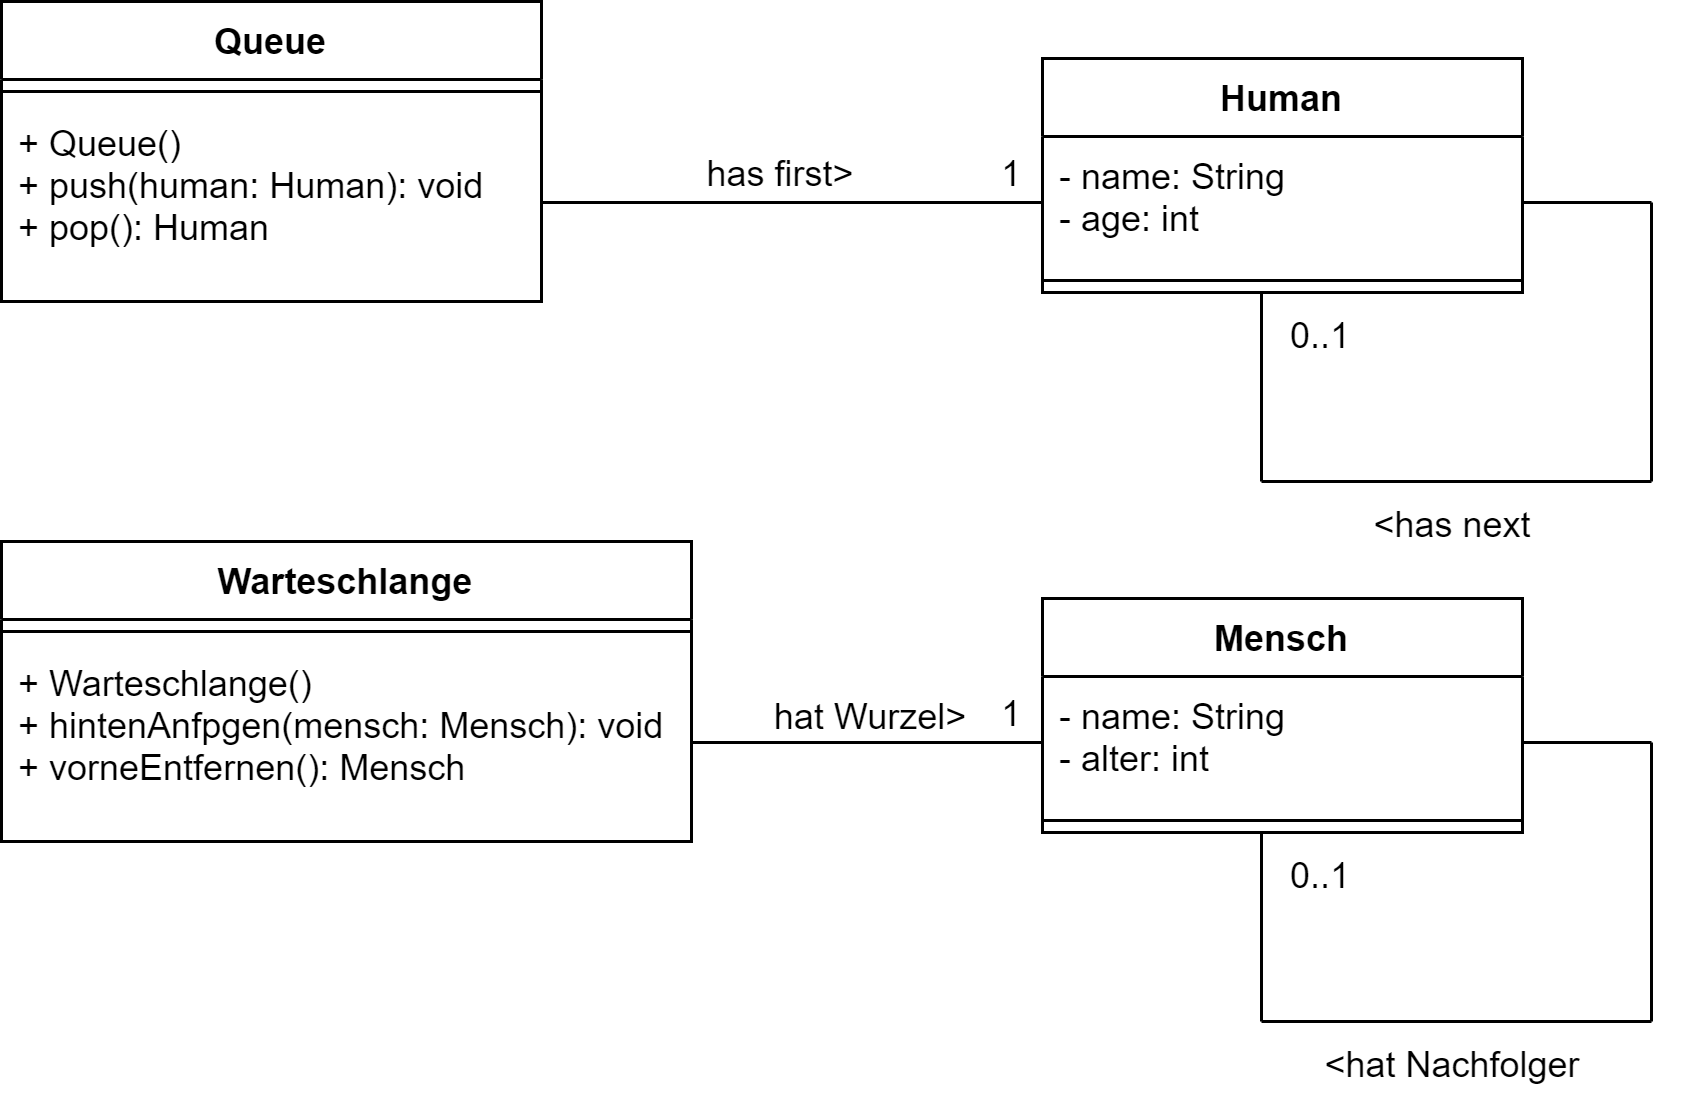
\includegraphics[scale=0.2]{../../media/linkedlist_diagram.png}
\end{center}
Bevor wir an der Implementierung arbeiten können muss zunächst ein neuer Begriff geklärt werden, die 
\textbf{\color{red} Rekursion}.
\newpage
\subsection{Rekursiv vs. Iterativ}
In der bisherigen Programmierung wurden fast ausschließlich \textbf{iterative} Algorithmen besprochen. 
Wollten wir alle Einträge eines Feldes durchlaufen schreiben wir z.B.: 
\begin{minted}{Java}
    for(int i = 0; i < array.length) {
        System.out.println(i);
    }
\end{minted}
Wir \q{zählen} von 0 bis zur Länge des Feldes hoch und arbeiten schrittweise weiter. In vielen Fällen 
ist eine iterative Arbeits- und Denkweise sinnvoll und entspricht auch unserer natürlichen Denkweise. \\
Sollen alle Zahlen von $1$ bis $5000$ aufsummiert werden, so können wir schreiben:
\begin{minted}{Java}
    result = 0;
    for(int i = 1; i <= 5000; i++) {
        result += i;
    }
\end{minted}
Typischerweise wird die Nützlichkeit der Rekursion mit Hilfe der Fibonacci-Folge (\href{https://de.wikipedia.org/wiki/Fibonacci-Folge}{Wikipedia Fibonacci}) 
verdeutlicht. Es ist eine Folge von Zahlen, die mit zwei Einsen beginnt und dann immer mit den letzten beiden
Zahlen das nächste Element der Folge berechnet, es gilt also: 
\begin{center}
    $f_n = f_{n-1} + f_{n-2}$ für $n\geq 3$
\end{center}
Damit ergibt sich die Folge:
\begin{center}
    $1, 1, 2, 3, 5, 8, 13, \dots$, da z.B. $13 = 8 + 5$
\end{center}
Ein iterativer Ansatz zur Berechnung der $n-$ten Zahl funktioniert mit Hilfe zweier Variablen, die die 
jeweils zwei letzten Ziffern speichern und daraus die neue berechnen: 
\begin{minted}{Java}
    public int fibonacci(int n) {
        if (n == 0)
            return 0;
        if (n == 1 || n == 2)
            return 1;

        int previous = 1;
        int result = 1;

        for (int i = 2; i < n; i++) {
            int sum = result + previous;
            previous = result;
            result = sum;
        }
        return result;
    }
\end{minted}
Dieser Code liefert uns die korrekten Ergebnisse. Fassen wir Fibonacci jedoch als Funktion auf, so 
könnte eine gewisse Systematik auffallen. Sei $f$ die abschnittsweise definierte Funktion, die die 
Fibonacci-Folge bauen soll, dann gilt: 
\begin{center}
    $f(0) = 0$ \\
    $f(1) = 1$ \\
    $f(n) = f(n-1) + f(n-2)$ für $n\geq 3$
\end{center}
Veranschaulicht man diese Vorschrift z.B. für $f(4)$, so erhält man: 
\begin{center}
    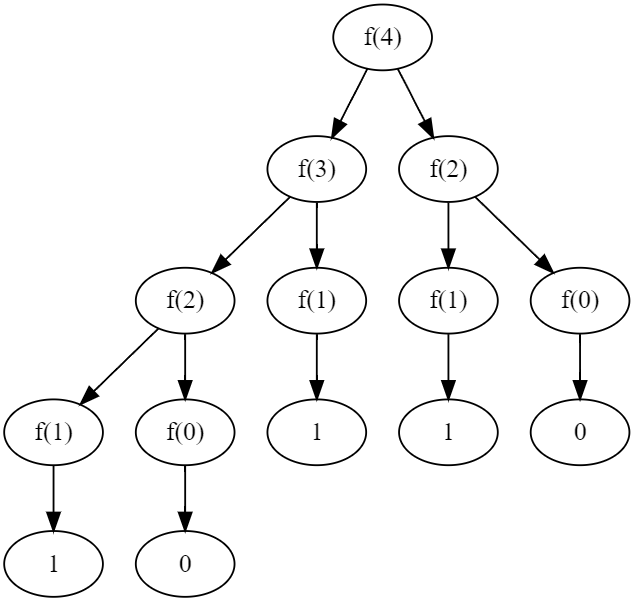
\includegraphics[scale=0.5]{../../media/graph_fib.png}
\end{center}
Zählt man nun die Anzahl der Einsen in der letzten Zeile zusammen, so kommt man auf die letztendliche
Lösung. Aber worauf basiert dieser Lösungsansatz? \\
Sieht man sich die Pyramide genauer an, so lässt sich erkennen, dass das Problem (die Berechnung 
von $f(4)$) schrittweise aufgeteilt wird. Dies geht nach bekannter Vorschrift immer so weiter, bis
man bei einem der \textbf{Basisfälle} ankommt. Die Basisfälle sind die einfachst möglichen 
Anwendungen der Regel. In diesem Fall die Funktionswerte der $0$ und der $1$. \\
Zusammengefasst könnte man sagen, dass die \textbf{Idee} der Rekursion darin besteht, das Problem
in kleine, überschaubare und leicht zu lösende Teil \textbf{aufzuteilen} und anschließend die 
Ergebnisse wieder zusammenzutragen.  \\
Im Sinne der Informatik lässt sich noch eine alternative Formulierung aufstellen. 
\begin{defi}[Rekursion]
Eine Methode wird als \textbf{rekursiv} bezeichnet, wenn sie sich selbst direkt oder indirekt
aufruft.
\end{defi}
\bsp 
\begin{minted}{Java}
    public void magic(int i){
        System.out.println("I was called " + i + " times");
        magic(i+1);
    }
\end{minted}
Führt man obigen Code aus, so erzeugt man natürlich eine Endlosschleife, bis irgendwann der 
Speicher vollgelaufen ist (oder der Compiler abbricht, weil er die Schleife erkannt hat). \\
Wichtig bei einer Rekursion ist es also eine \textcolor{blue}{\textbf{Abbruchbedingung}} zu haben. 
Im obigen Fall könnten wir die Funktion nur 100 mal aufrufen wollen:
\begin{minted}{Java}
    public void magic(int i){
        if(i > 100) {
            return;
        }
        System.out.println("I was called " + i + " times");
        magic(i+1);
    }
\end{minted}
Wir beenden mit dem return (Zurückgehen) die Kette der Methodenaufrufe, wenn der Übergabeparameter $i$ größer als 100 ist. \\ 
Zurück zu unserer Warteschlange. Die Tatsache, dass diese als \textbf{rekursive} Struktur 
gedacht ist sieht man schon am Klassendiagramm. Die Objekte der Klasse Mensch 
referenzieren jeweils ein Objekt derselben Klasse, 
das bedeutet aber, dass es keine Möglichkeit für die Warteschlange gibt mit einem iterativen 
Ansatz durch alle Menschen abzuarbeiten, wie das beim Feld-Ansatz der Fall war. Sie kann 
lediglich mit dem ersten Menschen in der Schlange interagieren. 
\begin{center}
    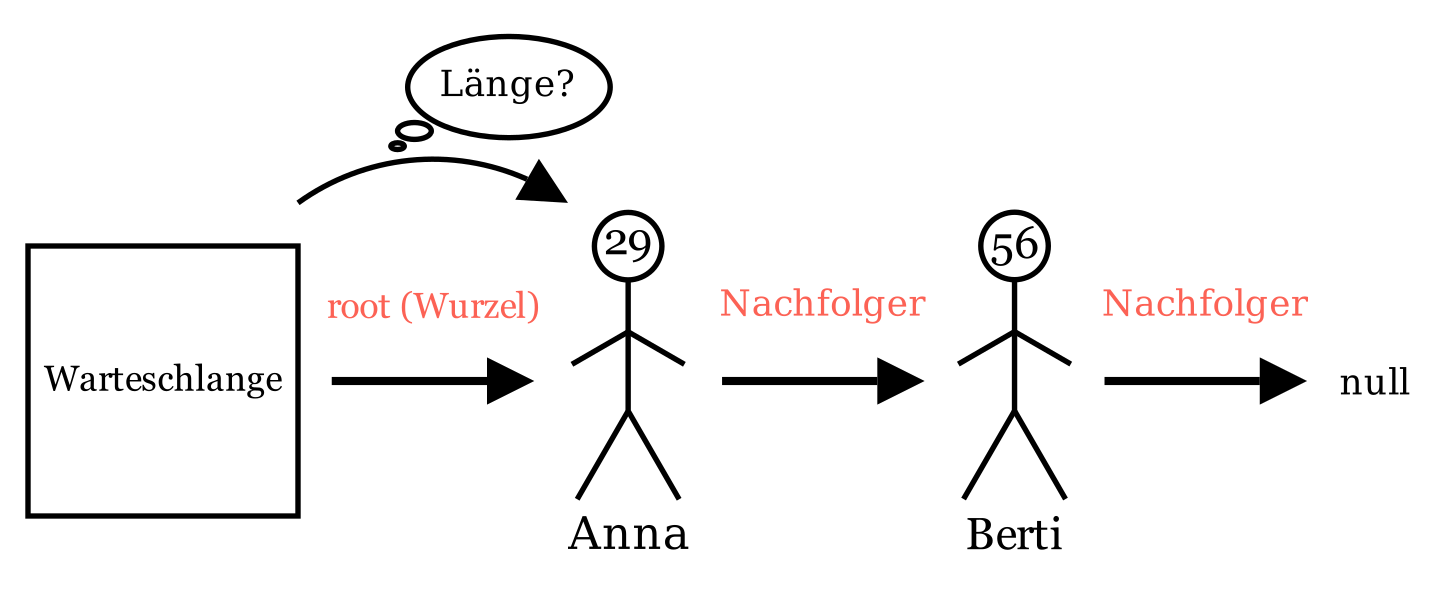
\includegraphics[scale = 0.25]{../../media/linked_list_length.png}
\end{center}
Möchten wir beispielsweise die Länge der Warteschlange wissen, so rufen wir eine Methode 
länge() auf der Warteschlange auf, die wiederum eine Methode länge() auf dem ersten Menschen
in der Schlange - in diesem Fall Anna - aufruft. \\
Anna allein kann die Länge aber ebenfalls nicht bestimmen, sie muss also Berti fragen und dazu 
(mithilfe ihrer Referenz zu Berti) auch die Methode länge() aufrufen. \\
\textit{Hinweis:} Hier kommt die Rekursion ins Spiel, wir rufen zwar nicht immer wieder auf 
demselben Objekt die Methode auf, allerdings wird die Methode länge() dennoch immer wieder 
aufgerufen! \\
Berti kann abschließend niemanden mehr fragen, denn er hat keinen Nachfolger, er antwortet 
also stattdessen mit $1$ an Anna. Sie wiederum zählt noch eins hinzu und gibt die - hier finale - 
Antwort $2$ an die Warteschlange zurück. Anschaulich gesprochen wurde also \q{von hinten} durchgezählt. 
\begin{center}
    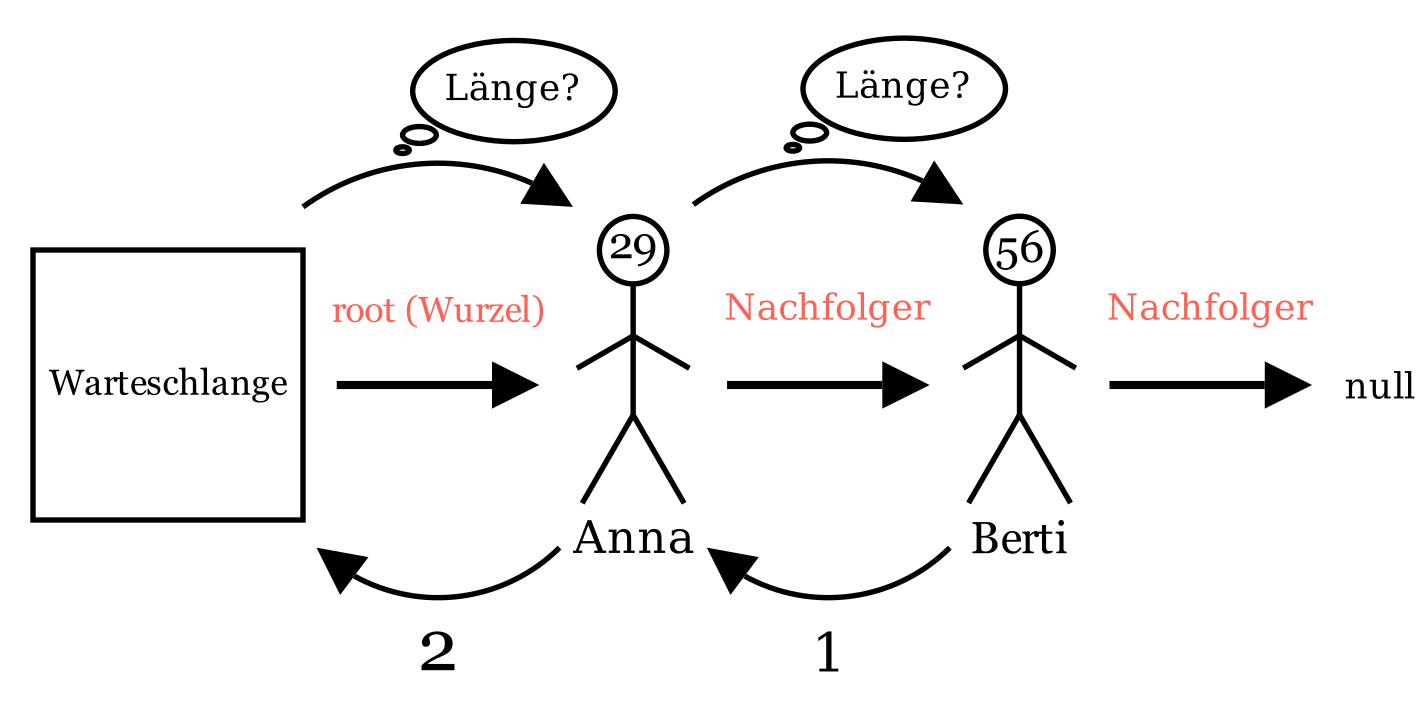
\includegraphics[scale = 0.20]{../../media/linked_list_length2.png}
\end{center}



\begin{task}{Rekursive Algorithmen}
    \\
    a) Schreiben Sie eine rekursive Methode, die den größten gemeinsamen Teiler zweier natürlicher Zahlen bestimmt. \\
    b) Schreiben Sie eine rekursive Methode, die das Problem der \q{Türme von Hanoi} löst \href{https://www.mathematik.ch/spiele/hanoi_mit_grafik/}{Türme von Hanoi}. Gehen Sie von einem Turm der Höhe 5 aus. 
\end{task}

\subsection{Implementierung}
Die konkrete Implementierung dieser Methode folgt in einem späteren Kapitel. Zunächst muss das
Grundgerüst geschaffen werden. Zur Erinnerung das Klassendiagramm, ergänzt um die Methode länge(), die
wir zusätzlich implementieren wollen. \\
\textit{Hinweis:} Die Methode länge() steht sowohl in der Klasse Warteschlange, als auch in der Klasse 
Mensch, da sie in beiden gebraucht wird. Das beide denselben Namen haben ist nicht zwingend notwendig,
der Übersichtlichkeit halber aber von Vorteil. 
\begin{center}
    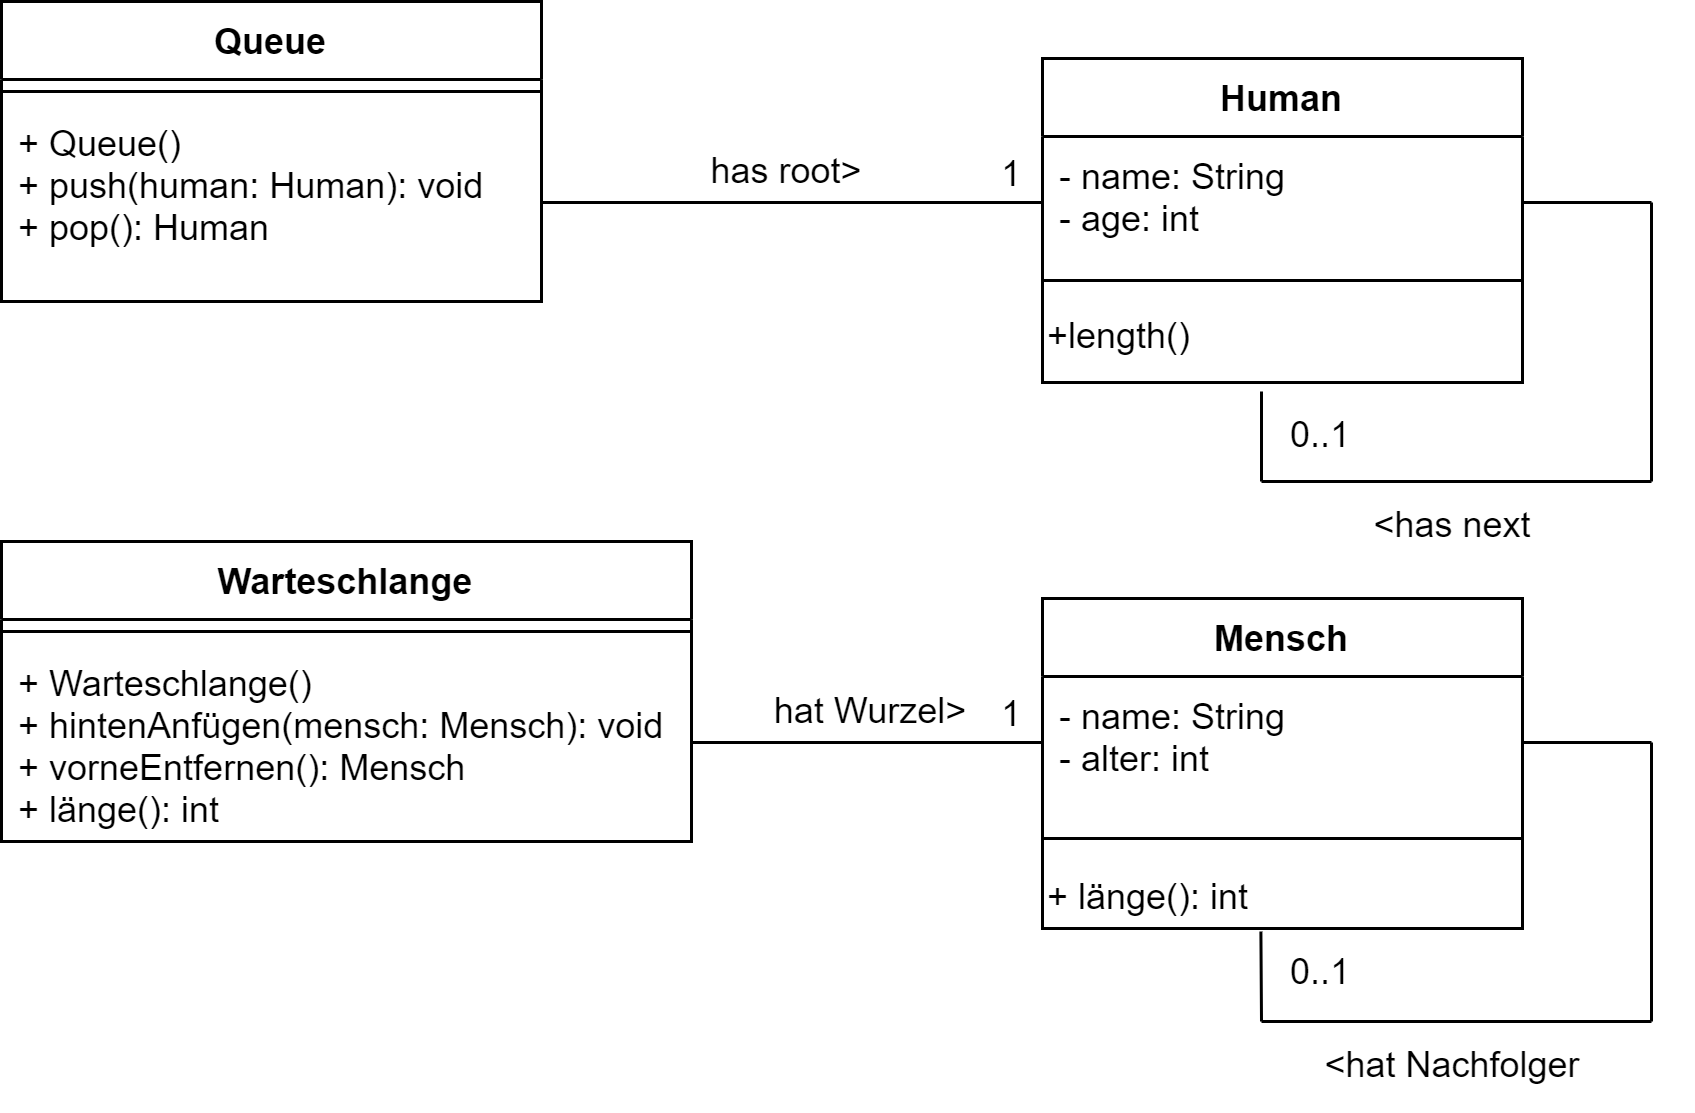
\includegraphics[scale=0.2]{../../media/linkedlist_diagram2.png}
\end{center}
Wir beginnen mit den Attributen und Konstruktoren:
\begin{minted}{Java}
    public class MyListLinked {
        private Human root;

        public MyListLinked() {
            root = null;
        }
    }

    public class Human() {
        private String name; 
        private int age;
        private Human next;

        public Human(String name, int age) {
            this.age = age;
            this.name = name;
            next = null;
        }
    }
\end{minted}
\textit{Hinweis:} Die explizite Definition von root und next als null ist nicht zwingend notwendig, 
erinnert aber daran, dass diese Attribute bei der Definition diesen Wert haben. \\
Bevor wir die Methoden zum Anfügen und Entfernen schreiben beginnen wir mit der Länge der Liste, um die 
Rekursion an einem typischen Beispiel besser zu verstehen, 
wir nehmen also an, wir hätten eine Liste, deren Länge wir prüfen können. \\
In der Klasse der Warteschlange selbst ist die Methode sehr einfach: 
\begin{minted}{Java}
    //class MyListLinked
    public int length(){
        if(root != null) {
            return root.length();
        } else {
            return 0;
        }
    }
\end{minted}
Wir rufen auf der uns bekannten Wurzel die Methode länge() auf und geben das Ergebnis zurück. Der interessante
Teil beginnt in der Klasse Mensch: 
\begin{minted}{Java}
    //class Human
    public int length() {
        if(next == null) {
            return 1;
        } else {
            return next.length() + 1;
        }
    }
\end{minted}
Die erste Bedingung entspricht der Frage, ob es einen Nachfolger in der Schlange gibt. Ist das nicht der Fall, 
da unter der Referenz des Nachfolgers nur null zu finden ist, so \q{weiß} der Mensch, dass er der letzte in der Schlange 
ist und gibt als Antwort an den vorletzten Menschen $1$ zurück (via return 1). \\
Der vorletzte Menschen (in unserem Beispiel weiter oben Anna) hatte aber nicht $null$ als Nachfolger. 
Deswegen wurde die Methode länge() auf dem Nachfolger aufgerufen, dieser Methodenaufruf hat $1$ zurückgegeben. 
Zu dieser $1$ wurde eine weitere $1$ hinzuaddiert und dann ebenfalls zurückgegeben. \\
Damit ist der länge()-Aufruf auf unserer Wurzel (Anna) beendet und die Warteschlange kann die Antwort 
($2$) ebenfalls zurückgeben. Noch einmal bildlich: 
\begin{center}
    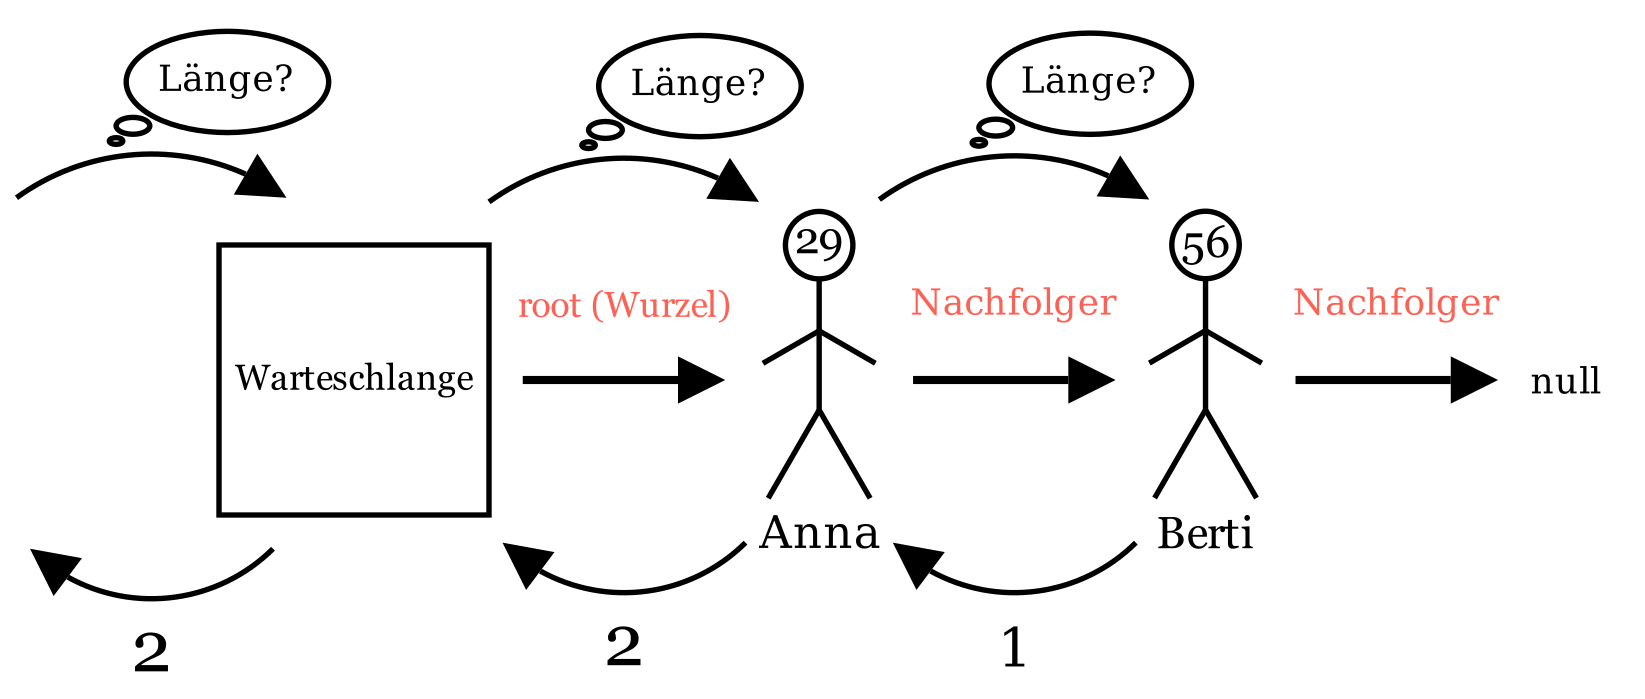
\includegraphics[scale = 0.20]{../../media/linked_list_length3.png}
\end{center}
Ein wenig formeller mit vier Menschen und in einem Sequenzdiagramm dargestellt:
\begin{center}
    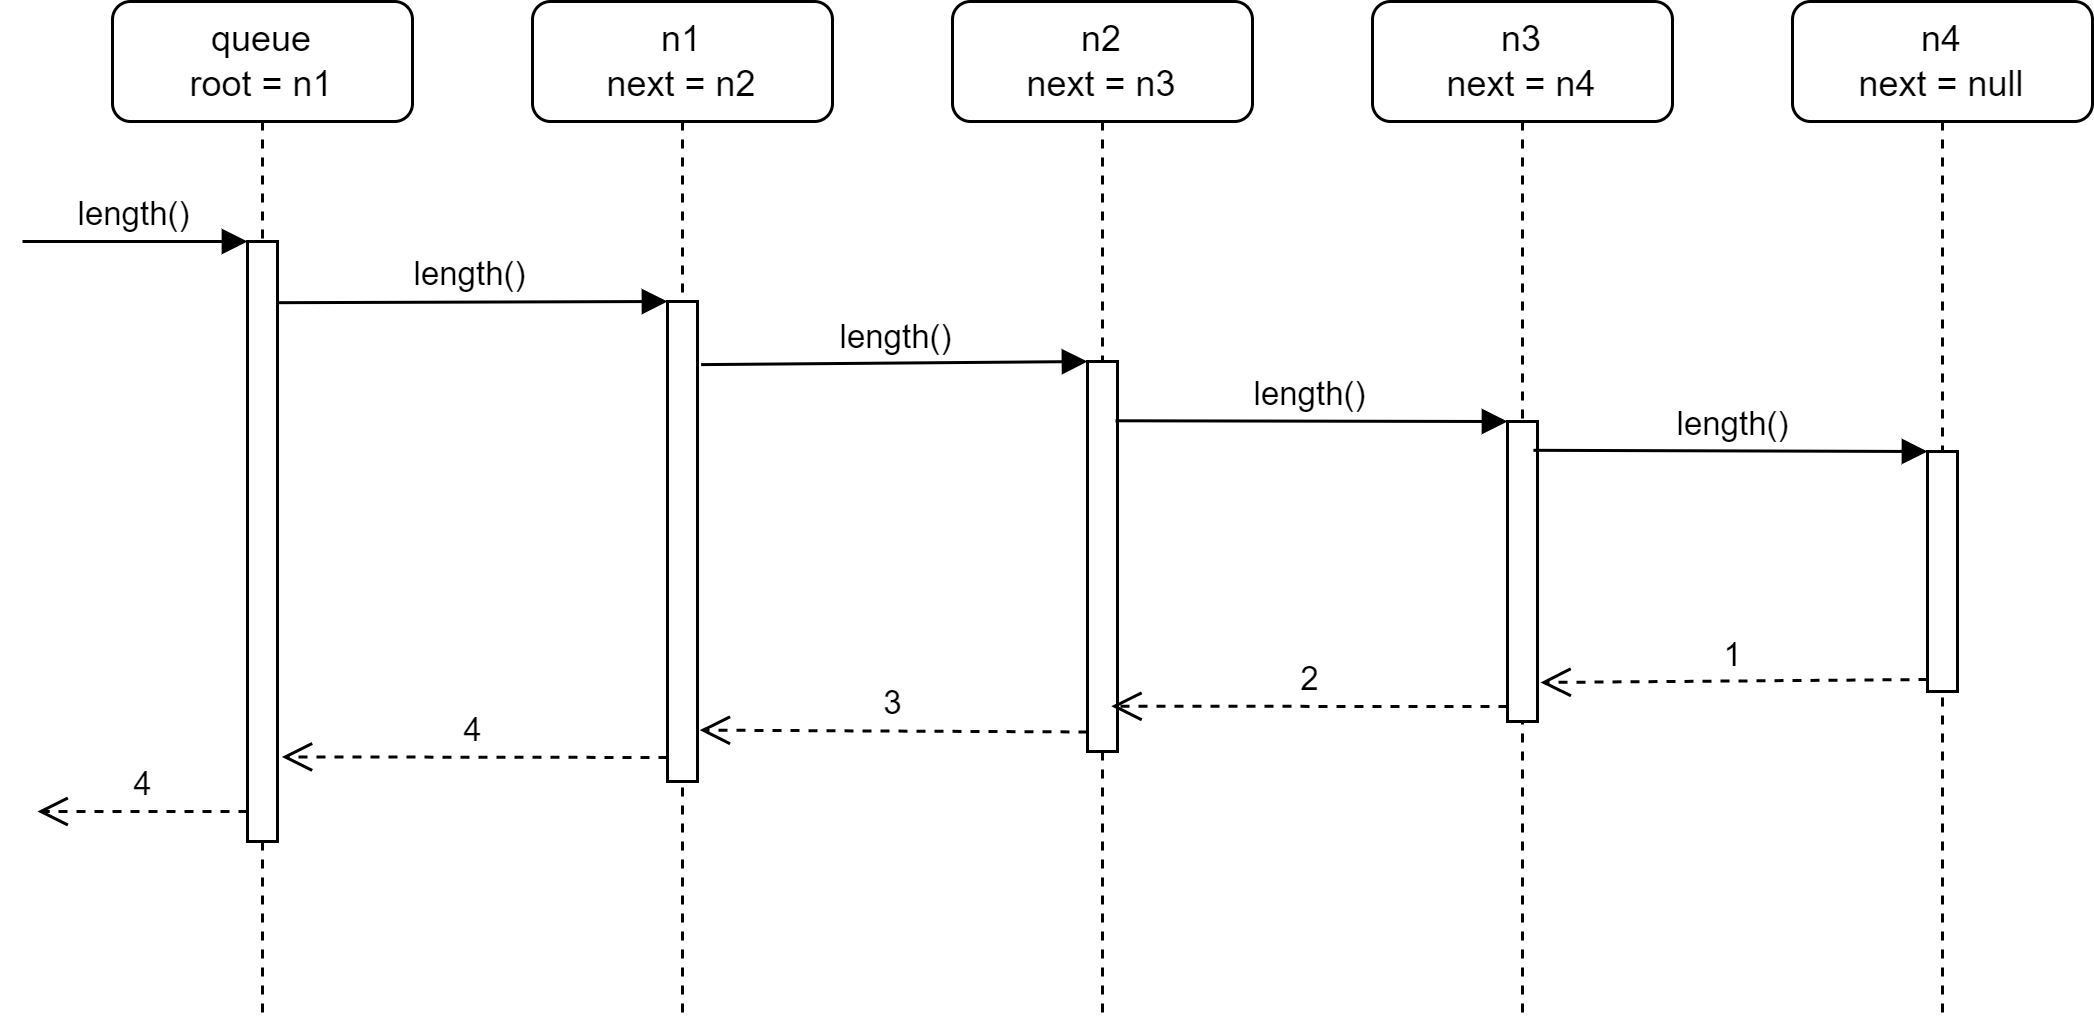
\includegraphics[scale = 0.20]{../../media/length_sequence.png}
\end{center}
Mit dieser Vorarbeit sollten die anderen beiden Methoden kein Problem mehr darstellen. Für die hintenAnfügen() Methode 
müssen wir nicht einmal einen Rückgabewert (und damit eine Abbruchbedingung) angeben. Wir wenden dieselbe Logik wie zuvor an:
\begin{minted}{Java}
    //class MyListLinked
    public void push(Human human) {
        if(root == null) {
            root = human;
        } else {
            root.push(human);
        }
    }
\end{minted}
In der Warteschlangen-Klasse wird wieder nur auf der Wurzel die hintenAnfügen() Methode ausgeführt, sofern diese 
existiert, andernfalls ist der übergebene Mensch die neue Wurzel. \\
Die Implementierung in der Klasse Mensch dagegen sieht fast völlig identisch aus, wir prüfen wieder, ob der nächste 
Mensch vorhanden ist, falls nein ($null$), so setzen wir den übergebenen Menschen als Nachfolger, andernfalls 
wird auf dem Nachfolger rekursiv die gleiche Methode aufgerufen, bis wir den letzten in der Reihe gefunden haben:
\begin{minted}{Java}
    // class Human
    public void push(Human human) {
        if(next == null) {
            next = human;
        } else {
            next.push(human);
        }
    }
\end{minted}
\begin{task}{1}
    Begründen Sie, ob die Methode vorneEntfernen() rekursiv sein muss oder nicht. Implementieren Sie sie anschließend.
\end{task}
Die Methode muss nicht rekursiv sein. Es wird nur das vorderste Element entfernt, das bedeutet, dass nur das 
zweite Element als neue Wurzel gesetzt werden muss. \\
\textbf{Problem}: Aktuell können wir auf die Nachfolger-Referenz des ersten in der Schlange nicht zugreifen, da 
es privat implementiert ist. Wir brauchen also eine getter-Methode für den Nachfolger, ein entsprechender setter kann ebenfalls nicht schaden:
\begin{minted}{Java}
    //class Human
    public Human getNext() {
        return next;
    }

    public void setNext(Human human) {
        next = human;
    }
\end{minted}
Bei der Implementierung der vorneEntfernen() Methode muss noch darauf geachtet werden, dass die Warteschlange 
leer sein könnte:
\begin{minted}{Java}
    //class MyListLinked 
    public Human pop() {
        if(root == null) {
            return null;
        } else {
            Human toReturn = root;
            root = root.getNext();
            toReturn.setNext(null);
            return toReturn;
        }
    }
\end{minted}
Graphisch dargestellt (als Bild und \href{https://youtu.be/ceQII7Bn9ts}{hier} im Video):
\begin{center}
    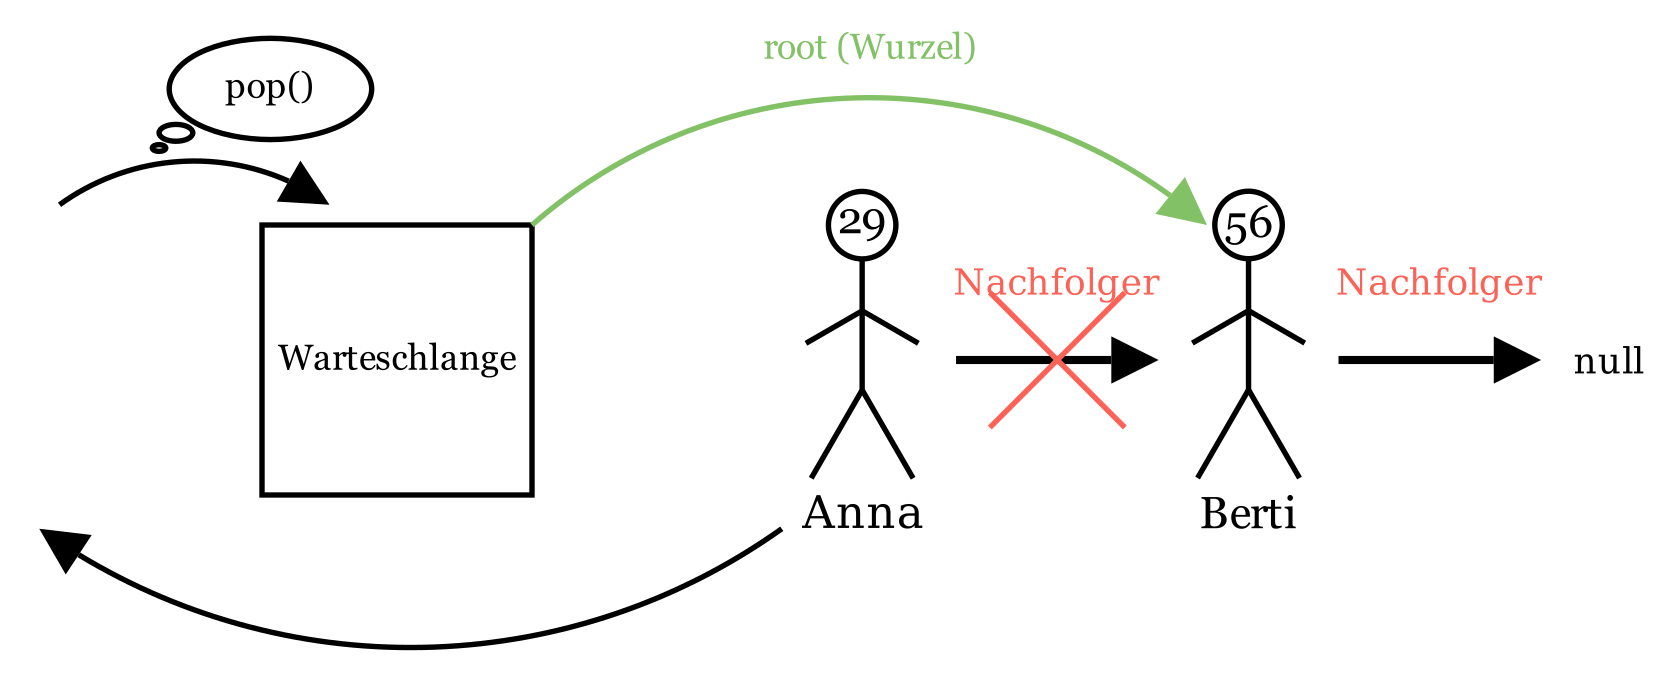
\includegraphics[scale = 0.2]{../../media/linked_list_pop.png}
\end{center}
Will man das zurückgegebene Objekt vom Typ Mensch weiter verwenden, so sollte die Referenz auf den 
Nachfolger dafür auf null gesetzt werden, da sonst die Liste nach der Entfernung weiter verändert werden könnte. \\
Die Methode muss allerdings nicht zwingend eine Referenz zur ehemaligen Wurzel zurückgeben. Lässt man die Rückgabe weg, so wird der garbage collector aktiv und entfernt das entsprechende Objekt. \\
Würde man die Null-Abfrage nicht schreiben, so gäbe es eine \textbf{null-pointer-exception}, wenn die Warteschlange 
leer ist. Das betreffende Program, dass die Anfrage stellt stürzt also ab. \\
Null-pointer-exceptions gehören zu den häufigsten Fehlern in objektorientierten Sprachen, die das Konzept der 
null enthalten. \\
\textbf{\textcolor{red}{Merke}}: Beim Entwickeln von Methoden müssen alle möglichen Spezialfälle (insbesondere der
Umgang mit Null-Referenzen) beachtet und entsprechend implementiert werden. \\

Versuchen Sie die folgenden Aufgaben zunächst selbstständig zu lösen, die Lösungen mit Erläuterungen finden sich dann auf 
den nächsten Seiten.

\begin{task}{2}
Implementieren Sie eine Methode nachHintenSetzen() (moveToBack()), die die Wurzel entfernt und an die letzte
Stelle setzt.
\end{task}

\begin{task}{3 - für Experten}
Erweitern Sie die Methode aus Aufgabe 2 so, dass die Position in der Warteschlange, an die die Wurzel geschoben wird, gewählt werden kann (moveBack(int position)).\\
\textit{Hinweis}: Die Methode soll \textbf{nicht} um die entsprechende Position nach hinten gerückt werden sondern  \textbf{an} diese Position in der Schlange gestellt werden.
\end{task}

\begin{task}{4}
    Schreiben Sie eine Methode schreibeListe() (printList), die die Warteschlange in einer sinnvollen Weise 
    auf der Konsole sichtbar macht. Formatieren Sie die Ausgabe ansprechend. \\
    Hinweis: Ergänzen Sie eine passende Methode in der Klasse Mensch (Human)!
\end{task}

\begin{task}{5}
    Verändern Sie die Methode aus Aufgabe 4 so, dass die Ausgabe nicht mehr auf die Konsole geschrieben wird, 
    sondern in einem String gespeichert wird, der am Ende zurückgegeben werden soll. 
\end{task}

\begin{task}{6 - für Experten}
    Schreiben Sie eine Methode sucheMenschInSchlange(Mensch m) (searchHumanInQueue(Human h)), die die Position 
    des Menschen in der Schlange zurückgibt. \\
    \textit{Hinweis}: Überschreiben Sie die allgemeine equals() Methode in der Klasse Mensch, wie bei der
    Feldimplementierung.
\end{task}

\begin{task}{7}
    Schreiben Sie eine Methode enthält(Mensch m) (contains(Human h)), die wahr zurückgibt, wenn 
    der entsprechende Mensch in der Schlange ist, anderfalls falsch. \\
    \textit{Hinweis}: Verwenden Sie wieder die equals-Methode aus Aufgabe 6.
\end{task}
\begin{task}{8 - für Experten}
    Schreiben Sie eine Methode entferneAnPosition(int position) (removeAtPosition(int position)), die den 
    Menschen an der gegebenen Stelle entfernt. Es soll eine Referenz zu diesem Menschen zurückgegeben werden. \\
\end{task}
\begin{task}{9}
    Schreiben Sie eine Methode zusammenfügen(MeineVerketteteListe zweiteWarteschlange) (concatenate(MyListLinked secondQueue)),
    die eine zusammengefügte Liste zurückgibt. 
\end{task}
\begin{task}{10 - frei}
    Überlegen Sie sich eigene, sinnvolle weitere Methoden für die Warteschlangen-Implementierung.
\end{task}

\newpage

\end{document}